\documentclass[a4paper,14pt]{extarticle}

% Путь до папки с общими шаблонами
\newcommand{\pathToCommonFolder}{/home/denilai/Documents/repos/latex/Common}
% Название работы в титуле
\newcommand{\workname}{Отчет по практической работе №4}
% Название дисциплины в титуле
\newcommand{\discipline}{Архитектура процессоров и микропроцессоров}
% Название кафедры в титуле
\newcommand{\kafedra}{Кафедра вычислительной техники}
% Тема работы в титуле
\newcommand{\theme}{Стадии выполнения команд процессором КР580ВМ80}
% Должность преподавателя в титуле
\newcommand{\rang}{cтарший преподаватель кафедры ВТ}
% ФИО преподавателя в титуле
\newcommand{\teacherfio}{Ю.~М.Скрябин}
\newcommand{\studentfio}{К.~Ю.~Денисов}
\newcommand{\signature}{\pathToCommonFolder/denisov-signature}

\newcommand{\pt}{PacketTracer\copyright}

\usepackage{tabularx}



\usepackage{booktabs}
\newcolumntype{b}{X}
\newcolumntype{s}{>{\hsize=.5\hsize}X}
\newcommand{\heading}[1]{\multicolumn{1}{|c|}{#1}}

% установка размера шрифта для всего документа
%\fontsize{20pt}{18pt}\selectfont
\usepackage{extsizes} % Возможность сделать 14-й шрифт

% Вставка заготовки преамбулы
% Этот шаблон документа разработан в 2014 году
% Данилом Фёдоровых (danil@fedorovykh.ru) 
% для использования в курсе 
% <<Документы и презентации в \LaTeX>>, записанном НИУ ВШЭ
% для Coursera.org: http://coursera.org/course/latex .
% Исходная версия шаблона --- 
% https://www.writelatex.com/coursera/latex/5.3

% В этом документе преамбула

% Для корректного использования русских символов в формулах
% пакеты hyperref и настройки, связанные с ним, стоит загуржать
% перед загрузкой пакета mathtext



% поддержка русских букв
% кодировка шрифта
%\usepackage[T2A]{fontenc} 
\usepackage{pscyr}

% использование ненумеровонного абзаца с добавлением его в содержаниеl

\newcommand{\anonsection}[1]{\section*{#1}\addcontentsline{toc}{section}{#1}}
\newcommand{\sectionunderl}[1]{\section*{\underline{#1}}}


% настройка окружения enumerate
\usepackage{enumitem}
\setlist{noitemsep}
\setlist[enumerate]{labelsep=*, leftmargin=1.5pc}

\usepackage{hyperref}

% сначала ставить \usepackage{extsizes} % Возможность сделать 14-й шрифт
% для корректной установки полей вставлять преамбулу следует в последнюю очередь (но перед дерективой замены \rmdefault)
\usepackage[top=20mm,bottom=25mm,left=35mm,right=20mm]{geometry} % Простой способ задавать поля

\hypersetup{				% Гиперссылки
	unicode=true,           % русские буквы в раздела PDF
	pdftitle={Заголовок},   % Заголовок
	pdfauthor={Автор},      % Автор
	pdfsubject={Тема},      % Тема
	pdfcreator={Создатель}, % Создатель
	pdfproducer={Производитель}, % Производитель
	pdfkeywords={keyword1} {key2} {key3}, % Ключевые слова
	colorlinks=true,       	% false: ссылки в рамках; true: цветные ссылки
	linkcolor=red,          % внутренние ссылки
	citecolor=black,        % на библиографию
	filecolor=magenta,      % на файлы
	urlcolor=blue           % на URL
}

%%% Работа с русским языком
\usepackage{cmap}					% поиск в PDF
\usepackage{mathtext} 				% русские буквы в формулах
\usepackage[T2A]{fontenc}			% кодировка
\usepackage[utf8]{inputenc}			% кодировка исходного текста
\usepackage[english,russian]{babel}	% локализация и переносы
\usepackage{indentfirst}
\frenchspacing

%для изменения названия списка иллюстраций
\usepackage{tocloft}


\renewcommand{\epsilon}{\ensuremath{\varepsilon}}
\renewcommand{\phi}{\ensuremath{\varphi}}
\renewcommand{\kappa}{\ensuremath{\varkappa}}
\renewcommand{\le}{\ensuremath{\leqslant}}
\renewcommand{\leq}{\ensuremath{\leqslant}}
\renewcommand{\ge}{\ensuremath{\geqslant}}
\renewcommand{\geq}{\ensuremath{\geqslant}}
\renewcommand{\emptyset}{\varnothing}

% Изменения параметров списка иллюстраций
\renewcommand{\cftfigfont}{Рисунок } % добавляем везде "Рисунок" перед номером
\addto\captionsrussian{\renewcommand\listfigurename{Список иллюстративного материала}}

\newcommand{\tm}{\texttrademark\ }
\newcommand{\reg}{\textregistered\ }


%%% Дополнительная работа с математикой
\usepackage{amsmath,amsfonts,amssymb,amsthm,mathtools} % AMS
\usepackage{icomma} % "Умная" запятая: $0,2$ --- число, $0, 2$ --- перечисление

%% Номера формул
%\mathtoolsset{showonlyrefs=true} % Показывать номера только у тех формул, на которые есть \eqref{} в тексте.
%\usepackage{leqno} % Нумереация формул слева

%% Свои команды
\DeclareMathOperator{\sgn}{\mathop{sgn}}

%% Перенос знаков в формулах (по Львовскому)
\newcommand*{\hm}[1]{#1\nobreak\discretionary{}
{\hbox{$\mathsurround=0pt #1$}}{}}


% отступ для первого абзаца главы или параграфа
%\usepackage{indentfirst}

%%% Работа с картинками
\usepackage{graphicx}  % Для вставки рисунков
\graphicspath{{images/}{screnshots/}}  % папки с картинками
\DeclareGraphicsExtensions{.pdf,.png,.jpg}
\setlength\fboxsep{3pt} % Отступ рамки \fbox{} от рисунка
\setlength\fboxrule{1pt} % Толщина линий рамки \fbox{}
\usepackage{wrapfig} % Обтекание рисунков текстом

%%% Работа с таблицами
\usepackage{array,tabularx,tabulary,booktabs} % Дополнительная работа с таблицами
\usepackage{longtable}  % Длинные таблицы
\usepackage{multirow} % Слияние строк в таблице

%%% Теоремы
\theoremstyle{plain} % Это стиль по умолчанию, его можно не переопределять.
\newtheorem{theorem}{Теорема}[section]
\newtheorem{proposition}[theorem]{Утверждение}

\theoremstyle{plain} % Это стиль по умолчанию, его можно не переопределять.
\newtheorem{work}{Практическая работа}[part]


 
 
\theoremstyle{definition} % "Определение"
\newtheorem{corollary}{Следствие}[theorem]
\newtheorem{problem}{Задача}[section]
 
\theoremstyle{remark} % "Примечание"
\newtheorem*{nonum}{Решение}



%%% Программирование
\usepackage{etoolbox} % логические операторы

%%% Страница

%	\usepackage{fancyhdr} % Колонтитулы
% 	\pagestyle{fancy}
%   \renewcommand{\headrulewidth}{0pt}  % Толщина линейки, отчеркивающей верхний колонтитул
% 	\lfoot{Нижний левый}
% 	\rfoot{Нижний правый}
% 	\rhead{Верхний правый}
% 	\chead{Верхний в центре}
% 	\lhead{Верхний левый}
%	\cfoot{Нижний в центре} % По умолчанию здесь номер страницы

\usepackage{setspace} % Интерлиньяж
\onehalfspacing % Интерлиньяж 1.5
%\doublespacing % Интерлиньяж 2
%\singlespacing % Интерлиньяж 1

\usepackage{lastpage} % Узнать, сколько всего страниц в документе.

\usepackage{soul} % Модификаторы начертания


\usepackage[usenames,dvipsnames,svgnames,table,rgb]{xcolor}


\usepackage{csquotes} % Еще инструменты для ссылок

%\usepackage[style=authoryear,maxcitenames=2,backend=biber,sorting=nty]{biblatex}

\usepackage{multicol} % Несколько колонок

\usepackage{tikz} % Работа с графикой
\usepackage{pgfplots}
\usepackage{pgfplotstable}

% модуль для вставки рыбы
\usepackage{blindtext}

\usepackage{listings}
\usepackage{color}


% для поворота отдельной страницы. Использовать окружение \landscape
\usepackage{pdflscape} 
\usepackage{rotating} 


\definecolor{mygreen}{rgb}{0,0.6,0}
\definecolor{mygray}{rgb}{0.5,0.5,0.5}
\definecolor{mymauve}{rgb}{0.58,0,0.82}


% пример импорта файла
%\lstinputlisting{/home/denilai/repomy/conf/distributions}

\lstset{
	language=Python,
	basicstyle=\footnotesize,        % the size of the fonts that are used for the code
	numbers=left,                    % where to put the line-numbers; possible values are (none, left, right)
	numbersep=5pt,                   % how far the line-numbers are from the code
	numberstyle=\tiny\color{mygray}, % the style that is used for the line-numbers
	stepnumber=2,                    % the step between two line-numbers. If it's 1, each line will be numbered
	% Tab - 2 пробела
	tabsize=2,    
	% Автоматический перенос строк
	breaklines=true,
	frame=single,
	breakatwhitespace=true,
	title=\lstname 
}



\author{Кирилл Денисов ИВБО-02-19}
\title{Практическая работа №6\\Вариант 6}
\date{\today}

\renewcommand{\withouttheme}{1}

% установка полуторного интервала
% \usepackage{setspace}  
% \onehalfspacing

% использовать Times New Roman
\renewcommand{\rmdefault}{ftm}


\begin{document}
	%\thispagestyle{empty}
	% Вставка первого титульного листа
	%%\newcommand{\withouttheme}{} добавить эту переменную для определения, нужна ли тема
%     {} - нужна
%    {1} - не нужна

%\newcommand{\withoutsubmissiondate}{} добавить эту переменную для определения, нужен ли срок предоставления отчета
%     {} - нужен
%    {1} - не нужен
\begin{center}
	\begin{figure}[h!]
		\begin{center}
		
\includegraphics[width=0.17\linewidth]{\pathToCommonFolder/gerb}
		%\caption{}\label{pic:first}
		%	\vspace{5ex}
		\end{center}	
	\end{figure}
 	\small	МИНОБРНАУКИ РОССИИ \\
	Федеральное государственное бюджетное образовательное учреждение\\
						высшего профессионального образования\\
\normalsize					
\textbf{«МИРЭА – Российский технологический университет»\\
						РТУ МИРЭА}\\
						\noindent\rule{1\linewidth}{1pt}\\
       Институт информационных технологий\\ %\vspace{2ex}
					\kafedra\\
		\vspace{3ex}
			\large \textbf{\workname}  \\
		%\vspace{1ex}
						по дисциплине\\ «\discipline» \\
		\vspace{3ex}
		\if \withouttheme
			\textbf{Тема работы:}\\ <<\theme>>
		\fi
\vspace{3ex}
\small
\begin{table}[h!]
\begin{tabular}{p{0.14\linewidth}p{0.38\linewidth}p{0.25\linewidth}p{0.2\linewidth}}
	\textbf{Выполнил:} & студент группы ИВБО-02-19 & \studentfio &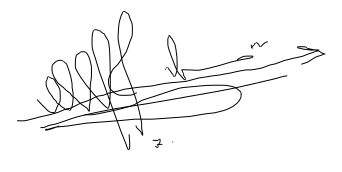
\includegraphics[width=0.8\linewidth]{\signature}\\ \\
	\textbf{Принял:} & \rang & \teacherfio 
\end{tabular}
\end{table}
\end{center}

\begin{flushleft}
	\begin{tabular}{p{0.25\linewidth}l}

		Работа выполена & <<\noindent\rule{2em}{1pt}>>
		                    \noindent\rule{5em}{1pt} 202\noindent\rule{1em}{1pt} \\

		<<Зачтено>> & <<\noindent\rule{2em}{1pt}>>
		\noindent\rule{5em}{1pt} 202\noindent\rule{1em}{1pt} \\

	\end{tabular}
\end{flushleft}

\normalsize
\begin{center}	
\vfill 
Москва 2021
\end{center}

	\newpage
	%\tableofcontents
	\newpage
	%\listoftables
\maketitle


\begin{mypart}{Преобразование IPv4-адресов из десятичной системы счисления с точкой -разделителем в двоичный формат}

	\begin{step}{Перевод числа из десятичной в двоичную систему счисления}
		\begin{table}[h!]
			\caption{Перевод чисел в двоичную систему}
			\centering
			\begin{tabular}{|c|c|}
				\hline
				\heading{\textbf{Десятичные}} &\heading{\textbf{Двоичные}}\\\hline
					192 & 11000000 \\ \hline
					168 & 10101000 \\\hline
					10 &      1010 \\\hline
					255 & 11111111 \\\hline
					2 &         10 \\\hline
			\end{tabular}
		\label{tab:ten2two}
		\end{table}
	\end{step}

	\begin{step}{Преобразование IPv4-адреса в двоичный формат}
		\begin{table}[h!]
			\caption{Преобразование IPv4-адреса в двоичный формат}
			\centering
			\begin{tabular}{|c|r|}
				\hline
				\heading{\textbf{Десятичные}} &\heading{\textbf{Двоичные}}\\\hline
				192.168.10.10   & 11000000.10101000.00001010.00001010 \\\hline
				209.165.200.229 & 11010001.10100101.11001000.11100101 \\\hline
				172.16.18.183   & 10101100.00010000.00010010.10110111 \\\hline
				10.86.252.17    & 00001010.01010110.11111100.00010001 \\\hline
				255.255.255.128 & 11111111.11111111.11111111.10000000 \\\hline
				255.255.192.0   & 11111111.11111111.11000000.00000000 \\\hline
			\end{tabular}
			\label{tab:ip-42two}
		\end{table}
	\end{step}
\end{mypart}

\begin{mypart}{Использование побитовой операции И для определения
		сетевых адресов}
	\begin{step}{Определение разрядности сетевого адреса}
		
		\begin{table}[h!]
			\caption{Преобразование IPv4-адреса в двоичный формат}
			\centering
			\begin{tabular}{|c|c|c|}
				\hline
				\textbf{Описание }&\textbf{Десятичные} &\textbf{Двоичные}\\\hline
				IP-адрес &      192.168.10.131  & 11000000.10101000.00001010.10000011\\\hline
				Маска подсети & 255.255.255.192 & 11111111.11111111.11111111.11000000\\\hline
				Сетевой адрес & 192.168.10.128  & 11000000.10101000.00001010.10000000\\\hline
			\end{tabular}
			\label{tab:web1}
		\end{table}
	
	\q Как определить, сколько бит нужно использовать для расчета сетевого адреса?
	
	\ans \textit{Перевести маску подсети в двоичный вид и посчитать количество единиц}
	
	\q Сколько бит в приведенном выше примере используется для расчета сетевого адреса?
	
	\ans \textit{26}			
	\end{step}

%\renewcommand{\labelenumi}{\asbuk{enumi})}
	\begin{step}{Определение сетевого адреса}
		
		\begin{enumerate}[label=\alph{enumi}) ]
			\item Введите отсутствующую информацию в таблицу ниже:
			
			\begin{table}[h!]
				\caption{Преобразование IPv4-адреса в двоичный формат. 1}
				\centering
				\begin{tabular}{|l|c|c|}
					\hline
					\textbf{Описание }&\textbf{Десятичные} &\textbf{Двоичные}\\\hline
					IP-адрес &      172.16.145.29  & 10101100.00010000.10010001.00011101\\\hline
					Маска подсети & 255.255.0.0    & 11111111.11111111.00000000.00000000\\\hline
					Сетевой адрес & 172.16.0.0     & 10101100.00010000.00000000.00000000\\\hline
				\end{tabular}
				\label{tab:web2}
			\end{table}
	
			\item Введите отсутствующую информацию в таблицу ниже:
			
			\begin{table}[h!]
				\caption{Преобразование IPv4-адреса в двоичный формат. 2}
				\centering
				\begin{tabular}{|l|c|c|}
					\hline
					\textbf{Описание }&\textbf{Десятичные} &\textbf{Двоичные}\\\hline
					IP-адрес &      192.168.10.10  & 11000000.10101000.00001010.00001010\\\hline
					Маска подсети & 255.255.255.0  & 11111111.11111111.11111111.00000000\\\hline
					Сетевой адрес & 172.16.0.0     & 11000000.10101000.00001010.00000000\\\hline
				\end{tabular}
				\label{tab:web3}
			\end{table}
				\newpage
			\item Введите отсутствующую информацию в таблицу ниже:
			
			\begin{table}[h!]
				\caption{Преобразование IPv4-адреса в двоичный формат. 3}
				\centering
				\begin{tabular}{|l|c|c|}
					\hline
					\textbf{Описание }&\textbf{Десятичные} &\textbf{Двоичные}\\\hline
					IP-адрес &      192.168.68.210  & 111000000.10101000.01000100.11010010\\\hline
					Маска подсети & 255.255.255.128  & 11111111.11111111.11111111.10000000\\\hline
					Сетевой адрес & 192.168.68.128     & 11000000.10101000.01000100.10000000\\\hline
				\end{tabular}
				\label{tab:web4}
			\end{table}

			\item Введите отсутствующую информацию в таблицу ниже:
			
			\begin{table}[h!]
				\caption{Преобразование IPv4-адреса в двоичный формат. 4}
				\centering
				\begin{tabular}{|l|c|c|}
					\hline
					\textbf{Описание }&\textbf{Десятичные} &\textbf{Двоичные}\\\hline
					IP-адрес &      172.16.188.15   & 10101100.00010000.10111100.00001111\\\hline
					Маска подсети & 255.255.240.0   & 11111111.11111111.11110000.00000000\\\hline
					Сетевой адрес & 172.16.176.0     & 10101100.00010000.10110000.00000000\\\hline
				\end{tabular}
				\label{tab:web5}
			\end{table}
		
			\item Введите отсутствующую информацию в таблицу ниже:
			
			\begin{table}[h!]
				\caption{Преобразование IPv4-адреса в двоичный формат. 5}
				\centering
				\begin{tabular}{|l|c|c|}
					\hline
					\textbf{Описание }&\textbf{Десятичные} &\textbf{Двоичные}\\\hline
					IP-адрес &      10.172.2.8   & 00001010.10101100.00000010.00001000\\\hline
					Маска подсети & 255.224.0.0   & 00001010.10101100.00000010.00001000\\\hline
					Сетевой адрес & 172.16.176.0     & 00001010.10100000.00000000.00000000\\\hline
				\end{tabular}
				\label{tab:web6}
			\end{table}
		
		\end{enumerate}
	\end{step}
\end{mypart}

\begin{mypart}{Применение расчетов сетевых адресов}
	\begin{step}{Определение подсетей по IP-v4}
		
		\begin{enumerate}[label=\alph{enumi})]
			\item 
			Вы настраиваете два ПК для своей сети. 
			
			Компьютеру PC-A присвоен IP-адрес \textit{192.168.1.18}.
			
			Компьютеру PC-B — IP-адрес \textit{192.168.1.33}. 
			
			Маска подсети обоих компьютеров — \textit{255.255.255.240}
			
			\q Какой сетевой адрес у PC-A? 
			
			\ans \textit{192.168.1.16}
			
			\q Какой сетевой адрес у PC-B? 
			
			\ans \textit{192.168.1.32}
			
			\q Смогут ли эти ПК взаимодействовать друг с другом напрямую? 
			
			\ans \textit{Нет, они находятся в разных подсетях}.
			
			\q Какой наибольший адрес, присвоенный компьютеру PC-B, позволит ему находиться в одной сети с
			PC-A?
			
			\ans \textit{192.168.1.224}
			
			\item 
			Вы настраиваете два ПК для своей сети. 
			
			Компьютеру PC-A присвоен IP-адрес \textit{10.0.0.16}.
			
			Компьютеру PC-B — IP-адрес \textit{10.1.14.68}. 
			
			Маска подсети обоих компьютеров — \textit{255.254.0.0}.
			
			\q Какой сетевой адрес у PC-A? 
			
			\ans \textit{10.0.0.0}
			
			\q Какой сетевой адрес у PC-B? 
			
			\ans \textit{10.0.0.0}
			
			\q Смогут ли эти ПК взаимодействовать друг с другом напрямую? 
			
			\ans \textit{Да, они находятся в одной подсети}.
			
			\q Какой наибольший адрес, присвоенный компьютеру PC-B, позволит ему находиться в одной сети с
			PC-A?
			
			\ans \textit{10.0.0.1}
		\end{enumerate}
	\end{step}

	\begin{step}{Установка адреса шлюза по умолчанию}
		\begin{enumerate}[label=\alph{enumi}) ]
			\item 
			В вашей компании действует политика использования первого IP-адреса в сети в качестве адреса
			шлюза по умолчанию. 
			
			Узел в локальной сети (LAN) имеет IP-адрес \textit{172.16.140.24} и маску подсети
			\textit{255.255.192.0}.
			
			\q Какой у этой сети сетевой адрес?
			
			\ans \textit{172.16.128.0}
			
			\q Какой адрес имеет шлюз по умолчанию для этого узла?
			
			\ans \textit{172.16.128.1}
			
			\item 
			В вашей компании действует политика использования первого IP-адреса в сети в качестве адреса
			шлюза по умолчанию. 
			
			Узел в локальной сети (LAN) имеет IP-адрес \textit{192.168.184.227} и маску подсети
			\textit{255.255.255.248}.
			
			\q Какой у этой сети сетевой адрес?
			
			\ans \textit{192.168.184.224}
			
			\q Какой адрес имеет шлюз по умолчанию для этого узла?
			
			\ans \textit{192.168.184.225}
		\end{enumerate}
	\end{step}
\end{mypart}

\begin{mypart}{Определение подсетей по IPv4-адресу}
	
	\begin{table}[htbp]
		\small
		\centering
		\caption{Определение подсетей по IPv4-адресу}
		\begin{tabular}{|c|c|p{0.24\linewidth}|p{0.13\linewidth}|p{0.13\linewidth}|}
			\hline
			
			\textbf{IPv4-
			адрес/префикс} & 
			
			\textbf{Сетевой адрес} & 
			\textbf{Широковещательный адрес} & \textbf{Общее количество бит узлов}& \textbf{Общее количество узлов} \\ \hline
			192.168.100.25/28 & 192.168.100.16 & 192.168.100.31 & 4 & 14 \\ \hline
			172.30.10.130/30 & 172.30.10.128 & 172.30.10.132 & 2 & 2 \\ \hline
			10.1.113.75/19 & 10.1.128.0 & 10.1.193.255 & 13 & 8190 \\ \hline
			198.133.219.250/24 & 198.133.219.0 & 198.133.219.255 & 8 & 254 \\ \hline
			128.107.14.191/22 & 128.107.12.0 & 128.107.15.255 & 10 & 1022 \\ \hline
			172.16.104.99/27 & 172.16.104.96 & 172.15.104.127 & 5 & 30 \\ \hline
		\end{tabular}
		\label{tab:subnets}
	\end{table}
	
\end{mypart}

\begin{mypart}{Расчет подсетей по IPv4-адресу}
	
	\begin{step}{Заполните приведенные ниже таблицы, зная заданный IPv4-адрес, исходную и
			новую маску подсети}
		
\begin{table}[h!]
		\caption{Расчет подсетей. 1}
		\centering
		\begin{tabular}{|l|l|}
			\hline
			\multicolumn{2}{|c|}{\textbf{Дано:}}  \\ \hline
			\multicolumn{ 1}{|l|}{\textbf{IP-адрес узла:}} & 192.168.200.139 \\ \hline
			\textbf{Исходная маска подсети:} & 255.255.255.0 \\ \hline
			\textbf{Новая маска подсети:} & 255.255.255.224 \\ \hline
			\multicolumn{2}{|c|}{\textbf{Найти:}}  \\ \hline
			\multicolumn{ 1}{|l|}{\textbf{Количество бит подсети}} & \multicolumn{1}{c|}{3}\\  \hline
			\textbf{Количество созданных подсетей} & \multicolumn{1}{c|}{8} \\ \hline
			\textbf{Количество бит узлов в подсети} & \multicolumn{1}{c|}{5} \\ \hline
			\textbf{Количество узлов в подсети} & \multicolumn{1}{c|}{30} \\ \hline
			\textbf{Сетевой адрес этой подсети} & 192.168.200.128 \\ \hline
			\textbf{IPv4-адрес первого узла в этой подсети} & 192.168.200.129 \\ \hline
			\textbf{IPv4-адрес последнего узла в этой подсети} & 192.168.200.158 \\ \hline
			\textbf{Широковещательный IPv4-адрес в этой подсети} & 192.168.200.159 \\ \hline
		\end{tabular}
		\label{}
	\end{table}


\begin{table}[h!]
		\centering
		\caption{Расчет подсетей. 2}
	\begin{tabular}{|l|l|}
		\hline
			\multicolumn{2}{|c|}{\textbf{Дано:}}  \\ \hline
		\textbf{IP-адрес узла:} & 10.101.99.228 \\ \hline
		\textbf{Исходная маска подсети:} & 255.0.0.0 \\ \hline
		\textbf{Новая маска подсети:} & 255.255.128.0 \\ \hline
			\multicolumn{2}{|c|}{\textbf{Найти:}}  \\ \hline
		\textbf{Количество бит подсети} & \multicolumn{1}{c|}{9} \\ \hline
		\textbf{Количество созданных подсетей} & \multicolumn{1}{c|}{512} \\ \hline
		\textbf{Количество бит узлов в подсети} & \multicolumn{1}{c|}{15} \\ \hline
		\textbf{Количество узлов в подсети} & \multicolumn{1}{c|}{32766} \\ \hline
		\textbf{Сетевой адрес этой подсети} & 10.101.0.0 \\ \hline
		\textbf{IPv4-адрес первого узла в этой подсети} & 10.101.0.1 \\ \hline
		\textbf{IPv4-адрес последнего узла в этой подсети} & 10.101.127.254 \\ \hline
		\textbf{Широковещательный IPv4-адрес в этой подсети} & 10.101.127.255 \\ \hline
	\end{tabular}
	\label{}
\end{table}

\begin{table}[h!]
		\centering
		\caption{Расчет подсетей. 3}
	\begin{tabular}{|l|l|}
		\hline
			\multicolumn{2}{|c|}{\textbf{Дано:}}  \\ \hline
		\textbf{IP-адрес узла:} & 172.22.32.12 \\ \hline
		\textbf{Исходная маска подсети:} & 255.255.0.0 \\ \hline
		\textbf{Новая маска подсети:} & 255.255.224.0 \\ \hline
			\multicolumn{2}{|c|}{\textbf{Найти:}}  \\ \hline
		\textbf{Количество бит подсети} & \multicolumn{1}{c|}{3} \\ \hline
		\textbf{Количество созданных подсетей} & \multicolumn{1}{c|}{8} \\ \hline
		\textbf{Количество бит узлов в подсети} & \multicolumn{1}{c|}{13} \\ \hline
		\textbf{Количество узлов в подсети} & \multicolumn{1}{c|}{8190} \\ \hline
		\textbf{Сетевой адрес этой подсети} & 172.22.0.0 \\ \hline
		\textbf{IPv4-адрес первого узла в этой подсети} & 172.22.0.1 \\ \hline
		\textbf{IPv4-адрес последнего узла в этой подсети} & 172.22.31.254 \\ \hline
		\textbf{Широковещательный IPv4-адрес в этой подсети} & 172.22.31.255 \\ \hline
	\end{tabular}
	\label{}
\end{table}


\begin{table}[h!]
	\centering
	\caption{Расчет подсетей. 4}
	\begin{tabular}{|l|l|}
		\hline
			\multicolumn{2}{|c|}{\textbf{Дано:}}  \\ \hline
		\textbf{IP-адрес узла:} & 192.168.1.245 \\ \hline
		\textbf{Исходная маска подсети:} & 255.255.255.0 \\ \hline
		\textbf{Новая маска подсети:} & 255.255.255.252 \\ \hline
			\multicolumn{2}{|c|}{\textbf{Найти:}}  \\ \hline
		\textbf{Количество бит подсети} & \multicolumn{1}{c|}{6} \\ \hline
		\textbf{Количество созданных подсетей} & \multicolumn{1}{c|}{64} \\ \hline
		\textbf{Количество бит узлов в подсети} & \multicolumn{1}{c|}{2} \\ \hline
		\textbf{Количество узлов в подсети} & \multicolumn{1}{c|}{2} \\ \hline
		\textbf{Сетевой адрес этой подсети} & 192.168.1.244 \\ \hline
		\textbf{IPv4-адрес первого узла в этой подсети} & 192.168.1.245 \\ \hline
		\textbf{IPv4-адрес последнего узла в этой подсети} & 192.168.1.246 \\ \hline
		\textbf{Широковещательный IPv4-адрес в этой подсети} & 192.168.1.247 \\ \hline
	\end{tabular}
	\label{}
\end{table}


\begin{table}[h!]
	\centering
	\caption{Расчет подсетей. 5}
	\begin{tabular}{|l|l|}
		\hline
			\multicolumn{2}{|c|}{\textbf{Дано:}}  \\ \hline
		\textbf{IP-адрес узла:} & 128.107.0.55 \\ \hline
		\textbf{Исходная маска подсети:} & 255.255.0.0 \\ \hline
		\textbf{Новая маска подсети:} & 255.255.255.0 \\ \hline
			\multicolumn{2}{|c|}{\textbf{Найти:}}  \\ \hline
		\textbf{Количество бит подсети} & \multicolumn{1}{c|}{8} \\ \hline
		\textbf{Количество созданных подсетей} & \multicolumn{1}{c|}{256} \\ \hline
		\textbf{Количество бит узлов в подсети} & \multicolumn{1}{c|}{8} \\ \hline
		\textbf{Количество узлов в подсети} & \multicolumn{1}{c|}{254} \\ \hline
		\textbf{Сетевой адрес этой подсети} & 128.107.0.0 \\ \hline
		\textbf{IPv4-адрес первого узла в этой подсети} & 128.107.0.1 \\ \hline
		\textbf{IPv4-адрес последнего узла в этой подсети} & 128.107.0.254 \\ \hline
		\textbf{Широковещательный IPv4-адрес в этой подсети} & 128.107.0.255 \\ \hline
	\end{tabular}
	\label{}
\end{table}

\begin{table}[h]
	\centering
	\caption{Расчет подсетей. 6}
	\begin{tabular}{|l|l|}
		\hline
			\multicolumn{2}{|c|}{\textbf{Дано:}}  \\ \hline
		\textbf{IP-адрес узла:} & 192.135.250.180 \\ \hline
		\textbf{Исходная маска подсети:} & 255.255.255.0 \\ \hline
		\textbf{Новая маска подсети:} & 255.255.255.248 \\ \hline
			\multicolumn{2}{|c|}{\textbf{Найти:}}  \\ \hline
		\textbf{Количество бит подсети} & \multicolumn{1}{c|}{5} \\ \hline
		\textbf{Количество созданных подсетей} & \multicolumn{1}{c|}{32} \\ \hline
		\textbf{Количество бит узлов в подсети} & \multicolumn{1}{c|}{3} \\ \hline
		\textbf{Количество узлов в подсети} & \multicolumn{1}{c|}{6} \\ \hline
		\textbf{Сетевой адрес этой подсети} & 192.135.250.176 \\ \hline
		\textbf{IPv4-адрес первого узла в этой подсети} & 192.135.250.177 \\ \hline
		\textbf{IPv4-адрес последнего узла в этой подсети} & 192.135.250.183 \\ \hline
		\textbf{Широковещательный IPv4-адрес в этой подсети} & 192.135.250.184 \\ \hline
	\end{tabular}
	\label{}
	\end{table}
	\end{step}
\end{mypart}

\end{document}



